\documentclass[12pt, letterpaper]{article}
\usepackage{graphicx}
\usepackage[export]{adjustbox}
\usepackage[siunitx]{circuitikz}
\graphicspath{{images/}}
\title{The Integration of the AY-3-8910 with the 6502 Microprocessor}
\author{Strahinja Marinkovic}
\date{July 2023}
\begin{document}
\maketitle

\begin{abstract}
One of the most fundemental parts within a computer design is audio. It brings any software to life
and gives the user another dimension of interaction previously missing. To explore how computer systems
use audio, this paper will explore the utilization of the programmable sound generator (PSG), AY-3-8910 chip, with the eight bit 6502 microprocessor. It will also discuss the implementation of adding the AY-3-8910 into an already existing system and the challenges that come along with it. 
\end{abstract}

\newpage

\section{PSG Integration}
\subsection{AY-3-8910}
The impact of sound in a system is immense. It is a fundemental part of a computer like video is. Thus, implementing
a simple solution in an eight bit system can be a challenge. A solution is a programmable sound generator. For instance,
the AY-3-8910 which this paper will explore. This device is a "Large Scale Integrated Circuit which can produce a wide variety of complex sounds under software control.\footnote{From Datasheet}" It requires a single 5V power supply and TTL compatible clock. Becuase the PSG is a "bus oriented" system, it should be realitivly easy to implement with a 6502 microprocessor. The following shows the registers that are under software control:

\begin{figure}[h]
    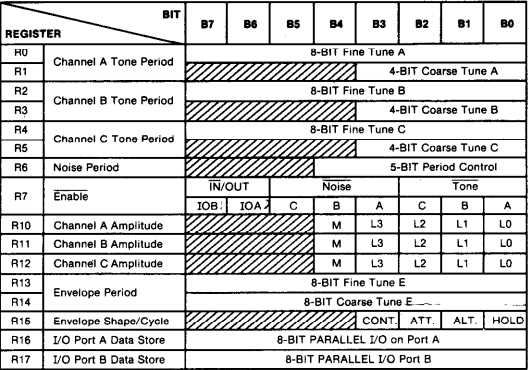
\includegraphics[width=0.75\textwidth, center]{psg_register_array}
    \caption{The memory layout of the AY-3-8910 registers. The register numbers are in octal.}
    \label{fig:registers_figure}
\end{figure}

The choice of the AY-3-8910 is very clear, compared to other sound generators, the AY-3-8910 has the ability to continue to perform sound effects while the processor is doing other tasks. After the initial commands have been sent by the MPU, it can execute other programs while letting sound to play and only have to update registers for a sound change.  Another nice feature of this chip is that it has three channels that can each be controlled, amplitude control, envelope shape, and two general purpose IO ports that can be used for anything. The pinout of the chip is as shown:

\begin{figure}[h]
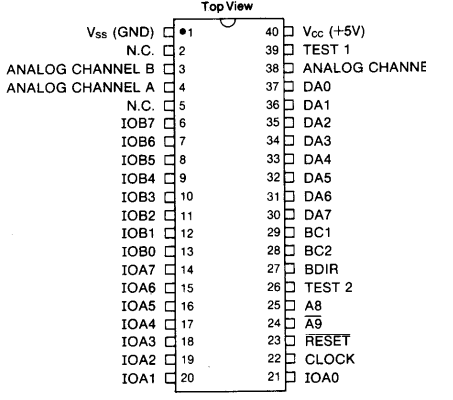
\includegraphics[width=0.5\textwidth, center]{pinout}
\caption{AY-3-8910 Pinout}
\label{fig:pinout_figure}
\end{figure}

Interfacing with this chip is quite simple. Data is written and read through the eight bit data/address bus, DA0 - DA7, with three control signals: BDIR, BC1, and BC2. There are no address lines as selecting register addresses occurs through the data bus. There are a total of 16 registers. Addresses are sent through the bus in addition to two extra bits acting as "chip selects" which come from pins A8 and A9. However, according to the data sheet, these are not totally necessary and even have their own pull up and pull down resistors respectively. However, I tied A8 to 5 volts through a 1K resistor and tied A9 to ground through a 1K resisitor just in case (the datasheet recommends it, especially in noisy environments). 
	
The control signals allow for four different functionalities: inactive, read, write, and latch. Inactive is when PSG to CPU bus is inactive and goes into a high impedence state. Read is for when the CPU reads from the PSG. Write is for when the CPU wants to write data to the PSG and latch is when the CPU writes an address to latch to a register. The following shows a table of these functions with the control signals.

\begin{center}
 \begin{tabular}{||c c c c||} 
 \hline
 BDIR & BC1 & BC2 & Function \\ [0.5ex] 
 \hline\hline
 0 & 0 & 1 & INACTIVE \\ 
 \hline
 0 & 1 & 1 & READ (FROM PSG) \\
 \hline
 1 & 0 & 1 & WRITE (TO PSG)\\
 \hline
 1 & 1 & 1 & LATCH ADDR \\
 \hline
\end{tabular}
\end{center}

This table shows how there are only two signals the MPU needs to control: BDIR and BC1. BC2 can be tied high through a resistor. However, before I can connect this PSG to the MPU, I will first go over how devices can be added to my 6502.

\subsection{6502 Device Interface}

Because the 6502 uses a bus oriented system, there must be a way to map devices to specific locations in memory. In my computer, I use a GAL chip to handle the memory mapping. The following is a table of the memory layout:


\begin{center}
\begin{tabular}{||c c||} 
 \hline
 Memory Range & Device \\ [0.5ex] 
 \hline\hline
 0x0000 - 0x7EFF & RAM (BANKED) \\ 
 \hline
 0x7F00 - 0x7FFF & IO \\
 \hline
 0x8000 - 0xFFFF & ROM \\
 \hline
\end{tabular}
\end{center}

Furthermore, the IO is broken up using a 4 to 16 line decoder. This means that from 0x7F00 to 0x7FF we can connect 16 devices each having 16 bytes of IO! For example, One of these lines is used to control a ACIA while two others are used to control two VIAS. This control line will be used for our decoding.
	
Now, one thing I noticed was that the BDIR control signal is in reference to if the MPU is either reading or writing. That means we can use the MPU's RWB pin. However, it is opposite of the PSG. According to the 6502's datasheet, a high on the RWB pin indicates a read and a low indicates a write. This is flipped from the PSG. For the control singal BC1, I decided to use address line A0 from the MPU. This way it uses different address locations for writing data and writing an address. However, the RWB and A0 can not be connected directly to the PSG as there is no way to control when the PSG bus is active or not.\footnote{We cannot connect the IO control line to BC2 because specific logic combinations from the datasheet with the control signal causes latching addresses outside of the PSG designated memory location.} I needed a way to flip the RWB control signal while also making sure that the bus was active in its memory location. 

\subsection{Solution}

A solution I thought of was using two NOR gates. A NOR gate is simply an OR gate with its output inverted. The following is its logic table:

\begin{center}
 \begin{tabular}{||c c c||} 
 \hline
 A & B & OUT \\ [0.5ex] 
 \hline\hline
 0 & 0 & 1 \\ 
 \hline
 0 & 1 & 0 \\
 \hline
 1 & 0 & 0 \\
 \hline
 1 & 1 & 0 \\
 \hline
\end{tabular}
\end{center}

\begin{figure}[h]
\centering
\begin{circuitikz}
 \draw 
node[american nor
port]{}
;
\end{circuitikz}
\caption{NOR Gate}
\end{figure}

The logic circuit for decoding uses two of these NOR gates for one AY-3-8910. One NOR gate's inputs are the IO control signal and RWB with its output connected to the BDIR control signal. The other NOR gate's inputs are again the IO control signal from the CPU and A0 with its output connected to BC1. Both NOR gates have the IO control as an input so that there is activity only in the designated memory location. The following is the logic table:

\begin{center}
\begin{tabular}{||c c c | c c | c||} 
 \hline
 IO & A0 & RWB & BDIR & BC1 & FUNCTION \\ [0.5ex] 
 \hline\hline
 0 & 0 & 0 & 1 & 1 & LATCH ADDRESS\\
\hline
 0 & 0 & 1 & 0 & 1 & READING FROM PSG\\ 
 \hline
 0 & 1 & 0 & 1 & 0 & WRITING TO PSG\\
 \hline
 0 & 1 & 1 & 0 & 0 & INACTIVE\\
 \hline
1 & 0 & 0 & 0 & 0 & INACTIVE \\
\hline
1 & 0 & 1 & 0 & 0 & INACTIVE \\
\hline
1 & 1 & 0 & 0 & 0 & INACTIVE \\
\hline
1 & 1 & 1 & 0 & 0 & INACTIVE \\
\hline
\end{tabular}
\end{center}

It can be seen that when IO is high, meaning it is inactive, the PSG bus is also inactive. Then, when IO is low, the CPU can either read or write or latch an address depending on if its in byte 0 or byte 1. This is extremely useful as it means that the PSG does not have to be controled by a VIA, which would take up 11 pins! A technique I tried prior to this was using the VIA but then connecting a second PSG to the firsts IO lines, this way they could be nested and only need 11 pins of the VIA. This can still work with the new set up or a different IO line can be connected to the second PSG since there are 16 lines to choose from meaning it would be difficult to run out. Otherwise the nesting technique for controlling them is also suitable.

\subsection{Circuit Layout}

The rest of the pins on the AY-3-8910 are quite simple to connect. Pin 23, RESET can be directly connected to the 6502 reset. Vss can be connected to ground and Vcc to 5 volts. Pin 22, CLOCK could be connected directly to the CPU's clock, however, the datasheet recommonds a clock speed of 2 MHz. In my system, I am using a clock speed of 1.8432 MHz because I have an ACIA that already requires that clock speed. 

The IO lines can be left unconnected, connected to a header or socket of some sort, or used to control other devices in your system like another PSG. The N.C and TEST pins are left unconnected. The AY-3-8910 has three analog channels. This means that there must be a circuit to merge these channels into one audio signal. The amplfication of the signal can depend on what speaker you use. In my case, the speakers I have do their own ampification thus I don't need to build my own. To get the analog channels together, I developed the circuit shown in figure \ref{channel_circuit}. It should be noted that this circuit does no amplification of the audio. It simply merges the channels together and does some filtering.

\begin{figure}[h]
\centering
\begin{circuitikz}
\draw (0,4)  to [short, -o] (0, 4) to[R, l=$R_1$,a=10K] ++(3, 0)
	++(-3,0) node[left](chA){$Channel_a$};
\node[circ] at (3,4) {};
\draw (0,2) to [short, -o] (0, 2) to[R, l=$R_2$,a=10K] ++(3, 0)
	++(-3,0) node[left](chB){$Channel_b$};
\node[circ] at (3,2) {};
\draw (0, 0) to [short, -o] (0, 0) to[R, l=$R_3$,a=10K]  ++(3, 0)
	++(-3,0) node[left](chC){$Channel_c$};
\node[circ] at (3,0) {};
\draw (3, 0) -- (3, 4);
\draw (3, 2) to [C, l = $C_1$, a=22pF] ++(3, 0);
\draw (3, 0) to [R, l = $R_4$, a=3.3K] ++(3, 0);
\draw (3, 4) to[C, l = $C_2$, a=10uF] (6, 4) to [short, -o] (6, 4) node[right](out){$Out$};
\draw (6, 2) -- (6, 0) node[ground]{};
\end{circuitikz}
\caption{Three to One Channel Circuit}
\label{channel_circuit}
\end{figure}

\subsection{Software}

The software that controls the PSG is quite simple. 

\newpage

\begin{thebibliography}{9}

\bibitem{datasheet}
General Instrument, "Programmable Sound Generator", AY-3-8910, 1978.

\bibitem{datasheet}
The Western Design Center Inc, "W65C02S 8–bit Microprocessor", W65C02S, 1983, [Revised Jan. 2022].


\end{thebibliography}

\end{document}
